\documentclass{beamer}
\usepackage{amsmath}
\usepackage[normalem]{ulem}
\usepackage{algorithm2e}
\usepackage{tikz}
\usepackage{array}
\usepackage{multirow}
\usepackage{xcolor}
\usepackage{mdframed}
\usepackage{scalerel}
\def\thumbsup{}   % To be removed
\def\thumbsdown{}  % To be removed
\newcommand{\tabitem}{~~\llap{\textbullet}~~}
\usetheme{Frankfurt}
\usecolortheme{seahorse}
\usepackage{graphicx}
\usepackage{calc}
\usepackage{tabu, mathtools}
\usepackage{enumitem}
\setitemize{label=\usebeamerfont*{itemize item}%
	\usebeamercolor[fg]{itemize item}
	\usebeamertemplate{itemize item}}

\newcommand\Wider[2][3em]{%
	\makebox[\linewidth][c]{%
		\begin{minipage}{\dimexpr\textwidth+#1\relax}
			\raggedright#2
		\end{minipage}%
	}%
}

\renewcommand*\footnoterule{}

\newcommand\blfootnote[1]{%
	\begingroup
	\renewcommand\thefootnote{}\footnote{#1}%
	\addtocounter{footnote}{-1}%
	\endgroup
}

\definecolor{PPorange}{RGB}{237,125,49}
\definecolor{PPgreen}{RGB}{112,173,71}
\definecolor{PPblue}{RGB}{91,155,213}

\newcolumntype{L}[1]{>{\raggedright\let\newline\\\arraybackslash\hspace{0pt}}m{#1}}
\newcolumntype{C}[1]{>{\centering\let\newline\\\arraybackslash\hspace{0pt}}m{#1}}
\newcolumntype{R}[1]{>{\raggedleft\let\newline\\\arraybackslash\hspace{0pt}}m{#1}}

\AtBeginSection{\frame{\sectionpage}} % This line enables sectiontitle-slides

\renewcommand{\footnotesize}{\scriptsize}

\title{Reinforcement Learning}
\author{M. Pl\"uss, E. Arnold}
\institute{
    University of Basel
}
\date{Mai 13, 2019}

\begin{document}
\maketitle


\section{Reinforcement Learning}
\subsection{subsec} % this enables bulletpoints at the top of the slide

\begin{frame}[c]{Reinforcement Learning - Idea}
\begin{itemize}
	\item Agent takes actions in an interactive environment (reward)
	\item Learning how good/bad actions are
	\item Goal: Maximize positive rewards
	\item Close relationship with biology, psychology and neuroscience
\end{itemize}
\begin{figure}[ht]
	\centering
	\includegraphics[width=0.9\textwidth]{img-elias/reinforcement_learning.png}
\end{figure}
\blfootnote{Image source: Sutton, Barto (1998)}
\end{frame}

\begin{frame}[c]{Reinforcement Learning - Example}
\begin{figure}[ht]
	\centering
	\includegraphics[width=0.9\textwidth]{img-elias/example.png}
\end{figure}
\blfootnote{Image source: A. Géron for Safari Books Online}
\end{frame}

\begin{frame}[c]{Difference to [Un-] Supervised-Learning}
\begin{itemize}
	\item Absence of an expert/teacher which labels input
	\item Agent has to distinguish good/bad behaviour by itself
	\item For that, the agent needs feedback from each state/input $\rightarrow$ \textbf{Reward} or \textbf{Reinforcement}
\end{itemize}
\begin{figure}[ht]
	\centering
	\includegraphics[width=0.9\textwidth]{img-elias/learningMethods.png}
	\caption{Reinforcement Learning compared to other learning strategies.}
	% Source: Wang et al. Machine Learning Algorithms in Bipedal Robot Control
\end{figure}
\blfootnote{Image source: Wang, Babuska (2012)}
\end{frame}

\begin{frame}[c]{Reminder - Grid World}
\begin{columns}[c]
	\column{.6\textwidth}
		\begin{itemize}
			\item Agent starts from (1,1) (start state)
			\item Every state $s$ gives a reward $R$ of $R(s)=-0.04$ except the goal states $R((4,3))=+1$ and $R((4,2))=-1$
			\item Transition probabilities:
				\begin{itemize}
					\item $80\%$ chance of desired direction
					\item $10\%$ chance of going left
					\item $10\%$ chance of going right
				\end{itemize}
		\end{itemize}
	\column{.4\textwidth}
	\begin{center}
		\includegraphics[width=0.9\linewidth]{img-elias/no_utilities.png}
	\end{center}
\end{columns}
\end{frame}

\begin{frame}[c]{Reminder - Terminology}
\begin{columns}[c]
	\column{.6\textwidth}
	\begin{itemize}
		\item \textbf{Trial}: One action sequence from the start state to a terminal state
		\item \textbf{Policy}: Instructions on which actions the agent should take in a given state (arrows)
		\begin{equation*}
			\text{Policy: }\pi(s) \rightarrow a
		\end{equation*}
	\end{itemize}
	\column{.4\textwidth}
	\begin{center}
		\includegraphics[width=0.9\linewidth]{img-elias/optimal_policy.png}
	\end{center}
\end{columns}
\end{frame}

\begin{frame}[c]{Agent design}
\Wider{
	\begin{table}[h]
		\tabulinesep=\tabcolsep
		\begin{tabu} to 12cm {X[3.2,c,m]X[2.8,c,m]X[6,c,m]}
			%\hline
			Utility-based Agent & \includegraphics[width=\linewidth,keepaspectratio]{img-elias/utility_based_agent.png} & \begin{itemize}[leftmargin=*]
				\item Calculations based on utility
				\item Needs state dependencies
			\end{itemize} \\ \hline
			Q-learning Agent & \includegraphics[width=\linewidth,keepaspectratio]{img-elias/q_learning_agent.png} & \begin{itemize}[leftmargin=*]
				\item Needs a list of applicable actions for each state
			\end{itemize} \\ \hline
			Reflex Agent & \includegraphics[width=\linewidth,keepaspectratio]{img-elias/reflex_agent.png} & \begin{itemize}[leftmargin=*]
				\item Reacts directly on percepts
				\item Bijection of states and actions
				\item E.g.: AI in a PONG-game
			\end{itemize} \\ %\hline
		\end{tabu}
	\end{table}
}
\end{frame}

\section{Passive Learning}
\subsection{subsec} % this enables bulletpoints at the top of the slide

\begin{frame}[c]{Passive Learning - Idea}
\begin{itemize}
		\item Simplest method to calculate a state's utility
		\item Fixed policy given
		\item Goal: Find utilities satisfying the \textbf{Bellman Equation}
		\item Similar to policy evaluation
		\item Difference: $P(s'|s,a)$ unknown $\rightarrow$ has to be learned
\end{itemize}
\vspace{1cm}
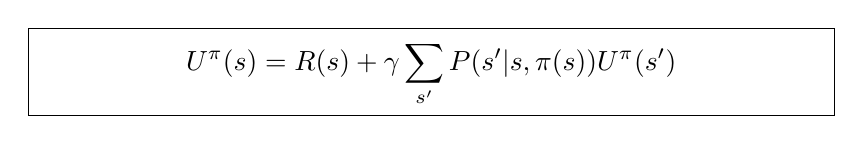
\begin{tikzpicture}
\node[draw,text width=10cm] (passive) at (0,0) {\begin{equation*}
	U^\pi(s)=R(s)+\gamma\sum_{s'}P(s'|s,\pi(s))U^\pi(s')
	\end{equation*}};
\end{tikzpicture}
%All learnung methods must satisfy the Bellman Equation
All learning methods converge to the Bellman Equation
\end{frame}

\begin{frame}[c]{Passive Learning - Direct Utility Estimation (DUE)}
\begin{columns}[c]
	\column{.55\textwidth}
	\begin{itemize}
		\item Let the Agent run a few trials
		\item $U^{\pi}(s)=\sum_{t=0}^{\infty}\gamma^{t}R(S_{t})$
		\item $S_{0}=s$
		\item Discount factor $\gamma$
		\item Reward-to-go
		\item Instance of supervised learning
		\item Keep running average
	\end{itemize}
	\column{.45\textwidth}
	\pause
		\includegraphics[width=0.9\linewidth]{img-elias/DUE_example.png}
		\begin{align*}
			U^{\pi}((1,1))&=\frac{\color{PPorange}(1-0.2)\color{black}+\color{PPgreen}(1-0.28)}{2}\\
			&=0.76\text{ (with }\gamma=1\text{)}
		\end{align*}
\end{columns}
\pause
\begin{center}
	\textit{Utilities are not independent!}
\end{center}
\end{frame}

\begin{frame}[c]{Passive Learning - Adaptive Dynamic Programming (ADP)}
\begin{itemize}
	\item Consider only local changes $\rightarrow$ recursive
	\item $U^{\pi}(s)=R(s)+\gamma\sum_{s'}[P(s'|s,\pi(s))*U^{\pi}(s')]$
	\item No independence assumption anymore
	%\item $P(s'|s,\pi(s))=\frac{N_{s'|sa}}{N_{sa}}$ learned from trials
	\item $P(s'|s,\pi(s))$ has to be learned from trials
\end{itemize}
\pause
\begin{columns}
	\column{.45\textwidth}
		\begin{center}
			\includegraphics[width=0.9\linewidth]{img-elias/ADP_example_passive.png}
		\end{center}
	\column{.3\textwidth}
		\begin{align*}
			U^{\pi}(X)=&-0.04\\
			+&\color{PPgreen}0.8*0.868\\
			+&\color{PPblue}0.1*0.762\\
			+&\color{PPorange}0.1*0.812\\
			=&0.811
		\end{align*}
	\column{.2\textwidth}
\end{columns}
\end{frame}


\begin{frame}[c]{Passive Learning - Temporal Difference Learning (TD)}
	\begin{itemize}
		\item Computationally cheaper than ADP
		\item No need for $P(s'|s,\pi(s))$
		\item ADP works with expected utility while
			  TD only works with 'observed' successor
		\item $U^{\pi}(s)=U^{\pi}(s)+\alpha (R(s)+\gamma U^{\pi}(s')-U^{\pi}(s))$
		\item $\alpha$: learning rate
	\end{itemize}
\end{frame}

\section{Active Learning}
\subsection{subsec} % this enables bulletpoints at the top of the slide

\begin{frame}[c]{Passive vs. Active Learning}
	\begin{center}
		\begin{tabular}{ c|c|c } 
		    & Passive Learning & Active Larning\\ \hline
			policy & given and fixed & none \\ \hline
			updates of $U(s)$ & after each trial & after each step \\ \hline
			considered actions & given by policy & all possible \\
		\end{tabular}
	\end{center}
	
	\vspace{.5cm}
	Bellmann equations: Passive-Learning $\rightarrow$ Active-Learning
	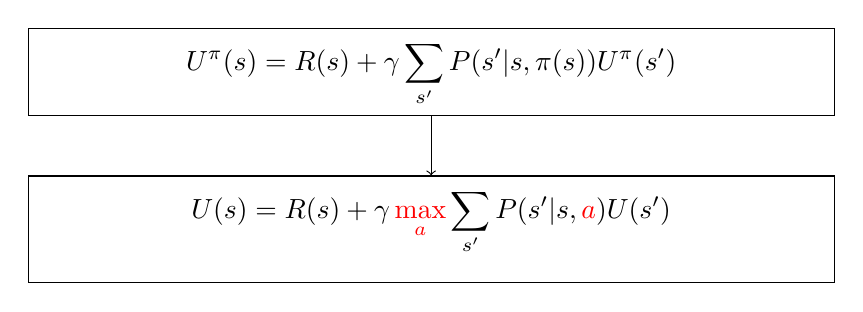
\begin{tikzpicture}
		\node[draw,text width=10cm] (passive) at (0,0) {\begin{equation*}
				U^\pi(s)=R(s)+\gamma\sum_{s'}P(s'|s,\pi(s))U^\pi(s')
			\end{equation*}};
		\node[draw,text width=10cm] (active) at (0,-2) {\begin{equation*}
				U(s)=R(s)+\gamma\color{red}\max_{a}\color{black}\sum_{s'}P(s'|s,\color{red}a\color{black})U(s')
			\end{equation*}};
		\draw [->] (passive) edge (active);
	\end{tikzpicture}
\end{frame}

%\begin{frame}[c]{Active Learning - Idea}
%\tabulinesep=\tabcolsep
%\begin{tabu} to 10cm {X[1.5,c,m] | X[7,c,m]}
%	Passive & 
%	\begin{tikzpicture}
%	\node (initial-1) at (0,0) {\includegraphics[width=0.35\linewidth]{img-elias/Passive_Active_a1.png}};
%	\node[draw, text width=2cm] (learn-1) at (2.75,0) {update\\utilities};
%	\node (optimal-1) at (5.5,0) {\includegraphics[width=0.35\linewidth]{img-elias/Passive_Active_p2.png}};
%	\draw [->] (initial-1) edge (learn-1);
%	\draw [->] (learn-1) edge (optimal-1);
%	\path[->,every loop/.style={looseness=3}] (learn-1) edge  [in=120,out=60,loop, above] node {trials} (); 
%	\end{tikzpicture}
%	\\ \hline
%	Active &
%	\begin{tikzpicture}
%	\node (initial-1) at (0,0) {\includegraphics[width=0.35\linewidth]{img-elias/Passive_Active_a1.png}};
%	\node[draw, text width=2cm] (learn-1) at (2.75,0) {update\\utilities and policy};
%	\node (optimal-1) at (5.5,0) {\includegraphics[width=0.35\linewidth]{img-elias/Passive_Active_a2.png}};
%	\draw [->] (initial-1) edge (learn-1);
%	\draw [->] (learn-1) edge (optimal-1);
%	\path[->,every loop/.style={looseness=3}] (learn-1) edge  [in=-120,out=-60,loop, below] node {steps} (); 
%	\end{tikzpicture}\\
%\end{tabu}
%\end{frame}


%\begin{frame}
%    \frametitle{Active Learning - Adaptive Dynamic Programming (ADP)}
%    \begin{itemize}
%    	\item Revisiting ADP
%    	\item Choose action which promises best outcome
%    	\item Formula of update rule same as Bellmann equation
%    \end{itemize}
%    
%	\begin{tikzpicture}
%		\node[draw,text width=10cm] (passive) at (0,0)		{\begin{equation*}
%			U^{\pi}(s)=R(s)+\gamma\sum_{s'}[P(s'|s,\pi(s))*U^{\pi}(s')]
%			\end{equation*}};
%		\node[draw,text width=10cm] (active) at (0,-2) {\begin{equation*}
%			U(s)=R(s)+\gamma\max_{a}\sum_{s'}[P(s'|s,a)*U(s')]
%			\end{equation*}};
%		\draw [->] (passive) edge (active);
%	\end{tikzpicture}
%\end{frame}

\begin{frame}[c]{Active Learning - Adaptive Dynamic Programming (ADP)}
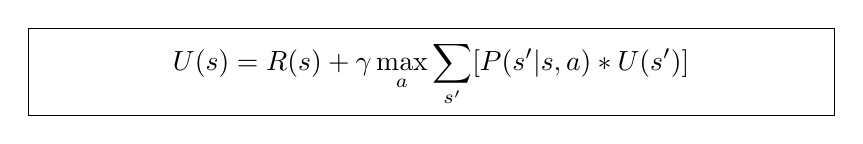
\begin{tikzpicture}
\node[draw,text width=10cm] (active) at (0,-2) {\begin{equation*}
	U(s)=R(s)+\gamma\max_{a}\sum_{s'}[P(s'|s,a)*U(s')]
	\end{equation*}};
\end{tikzpicture}
\begin{columns}
	\column{.5\textwidth}
	\begin{center}
		\includegraphics[width=\linewidth]{img-elias/ADP_example_active.png}
	\end{center}
	\column{.3\textwidth}
	\begin{align*}
	U^{\pi}(X)&=-0.04\\
	&\max_{a}(0.811,\\
	&\color{white}+\color{PPgreen}0.8*0.762\\
	&+\color{PPblue}0.1*0.868\\
	&+\color{PPorange}0.1*0.812\color{black})\\
	&=0.811
	\end{align*}
\end{columns}
\end{frame}


\begin{frame}
    \frametitle{Active Learning - Q-Learning}
    \begin{itemize}
    	\item Learning state-action pair utilities
    	\item $U(s) = max_{a}Q(s,a)$ where $Q(s,a)$ is state-action pair utility
	\end{itemize}
	
	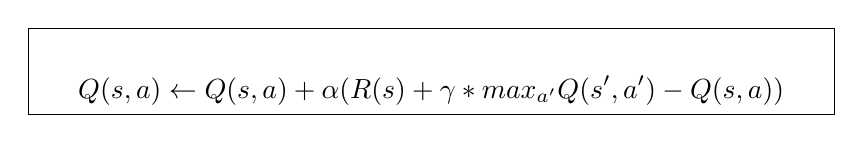
\begin{tikzpicture}
	\node[draw,text width=10cm] (q-learning) at (0,0) {
	\begin{equation*}
		Q(s,a) \leftarrow Q(s,a) + \alpha(R(s) + \gamma*max_{a'}Q(s',a') - Q(s,a))
	\end{equation*}
	};
	\end{tikzpicture}
	
	\begin{itemize}
		\item $\alpha$: learning factor
		\item $\gamma$: discount factor
		\item $s',a'$: states and actions that can be applied next
		\item Rating utility of state-action pair based on following state-action pair
	\end{itemize}
\end{frame}

\begin{frame}
    \frametitle{Active Learning - Q-Learning}
    
	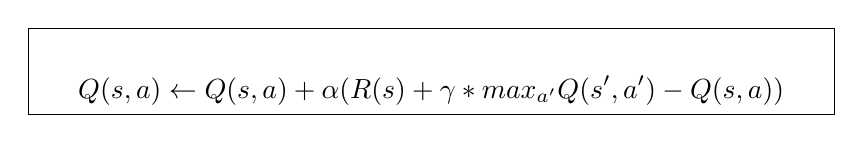
\begin{tikzpicture}
	\node[draw,text width=10cm] (q-learning) at (0,0) {
	\begin{equation*}
		Q(s,a) \leftarrow Q(s,a) + \alpha(R(s) + \gamma*max_{a'}Q(s',a') - Q(s,a))
	\end{equation*}
	};
	\end{tikzpicture}
	
	\begin{center}
		\includegraphics[width=0.6\linewidth]{img-michael/q_learning.png}
	\end{center}
\end{frame}

\section{Exploration vs. Exploitation}
\subsection{subsec} % this enables bulletpoints at the top of the slide

\begin{frame}[c]{Exploration vs. Exploitation}
\begin{itemize}
	\item Always choose the best looking action (one-step look-ahead)
	\item Initial policy = optimal policy
	\item Nevertheless, a sub-optimal policy is learned
\end{itemize}
	\begin{columns}[c]
		\column{.45\textwidth}
			\begin{figure}
				\includegraphics[width=0.9\linewidth]{img-elias/optimal_policy.png}
			\end{figure}
		\column{.45\textwidth}
		\begin{center}
			\includegraphics[width=0.9\linewidth]{img-elias/learned_policy.png}
		\end{center}
	\end{columns}
\begin{itemize}
	\item one-step look-ahead is not enough
	\item Need the ability to explore possible shortcuts
\end{itemize}
\end{frame}

\begin{frame}[c]{Exploration vs. Exploitation - GLIE}
	\begin{itemize}
		\item Solution: greedy in the limit of infinite exploration
		\begin{itemize}
			\item Start curious (much exploration)
			\item Chance to take random action instead of most attractive
			\item Achieved by giving those actions very high rewards $R^{+}$
			\item Decrease chance over time
		\end{itemize}
		\item Issue: when to switch from exploring to exploiting?
	\end{itemize}
	
	\begin{tikzpicture}
		\node (initial) at (0,0){\includegraphics[width=0.3\linewidth]{img-michael/policy_search_first_choice.png}};
		\node (modified) at (5.5,0) {\includegraphics[width=0.3\linewidth]{img-michael/exploration_reward.png}};
		\draw [->] (initial) edge (modified);
	\end{tikzpicture}
\end{frame}



\section{Generalization} 
\subsection{subsec} % this enables bulletpoints at the top of the slide

\begin{frame}
    \frametitle{Generalization - Idea}
    \begin{itemize}
    	\item State-spaces often large
    	\item Calculate utilities with parameters $\theta$
    	\item Function approximation
    	\item Learn parameters instead of utilities
	\end{itemize}
	
	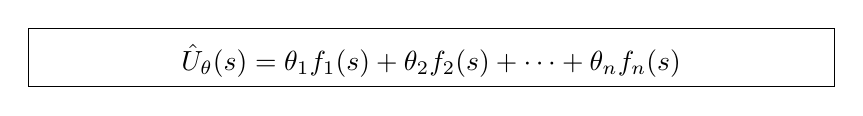
\begin{tikzpicture}
	\node[draw,text width=10cm] (approximation) at (0,0) {
	\begin{equation*}
		\hat{U}_{\theta}(s) = \theta_{1}f_{1}(s) + \theta_{2}f_{2}(s) + \cdots + \theta_{n}f_{n}(s)
	\end{equation*}
	};
	\end{tikzpicture}
\end{frame}

\begin{frame}
    \frametitle{Generalization - Example}
    \begin{itemize}
    	\item Grid world of size 20x20.
    	\item Goal state +1 in position (10,10)
	\end{itemize}

	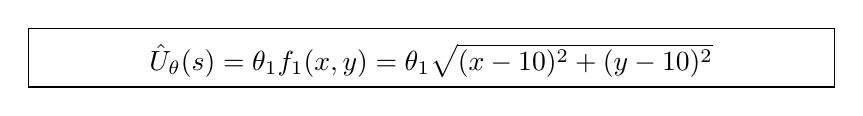
\begin{tikzpicture}
	\node[draw,text width=10cm] (example) at (0,0) {
	\begin{equation*}
		\hat{U}_{\theta}(s) = \theta_{1}f_{1}(x,y) = \theta_{1}\sqrt{(x-10)^2 + (y-10)^2}
	\end{equation*}
	};
	\end{tikzpicture}
	
	\begin{center}
		\includegraphics[width=0.4\linewidth]{img-michael/generalization_cone.png}
	\end{center}
\end{frame}

\begin{frame}
    \frametitle{Generalization - Update rule}
    \begin{itemize}
    	\item Widrow-Hoff rule or Delta rule
    	\item Adjust parameters after each trial
    \end{itemize}
    
	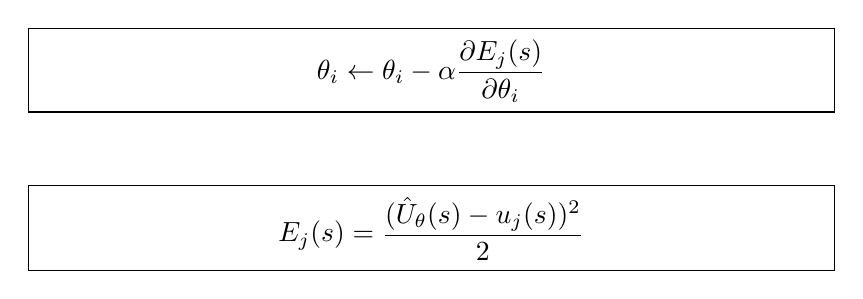
\begin{tikzpicture}
	\node[draw,text width=10cm] (update_rule) at (0,0) {
	\begin{equation*}
		\theta_{i} \leftarrow \theta_{i} - \alpha \frac{\partial E_{j}(s)} {\partial\theta_{i}}
	\end{equation*}
	};
	
	\node[draw,text width=10cm] (update_rule_sub) at (0,-2) {
	\begin{equation*}
		E_{j}(s) = \frac{(\hat{U}_{\theta}(s) - u_{j}(s))^2} {2}
	\end{equation*}
	};
	\end{tikzpicture}
	
    \begin{itemize}
    	\item $u_{j}(s)$: observed utility of state s in j-th trial
    	\item $\alpha$: learning factor
    	\item Leads to hill-climbing
    \end{itemize}
\end{frame}

\section{Policy Search} 
\subsection{subsec} % this enables bulletpoints at the top of the slide

\begin{frame}
    \frametitle{Policy Search - Idea}
    \begin{itemize}
    	\item Find a policy $\pi_{\theta}$ for state-space
    	\item Represent policy as parameterized formula
    	\item Like generalization, but parameters for action choice instead of utility calculation
    	\item Obvious policy: choose action which promises biggest reward $\rightarrow$ greedy agent
    \end{itemize}
\end{frame}

\begin{frame}
    \frametitle{Policy Search - Problems}
    \begin{itemize}
    	\item  $\pi_{\theta}$ often discontiuous function
    	\begin{itemize}
    		\item Slightly changed parameters $\rightarrow$ choose another action
    		\item Impossible to take derivative
    	\end{itemize}
    \end{itemize}
    
	\begin{center}
		\includegraphics[width=0.3\linewidth]{img-michael/policy_search_first_choice.png}
		\includegraphics[width=0.3\linewidth]{img-michael/policy_search_second_choice.png}
	\end{center}
	
    \begin{itemize}
    	\item Example: greedy agent
	\end{itemize}
\end{frame}

\begin{frame}
	\frametitle{Policy Search - Problems}
	\begin{itemize}
    	\item Solution: stochastic policy representation
    \end{itemize}
    
    Softmax function:
    
	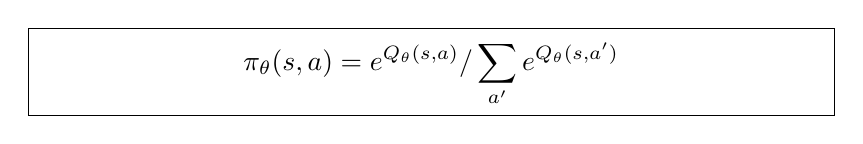
\begin{tikzpicture}
	\node[draw,text width=10cm] (softmax) at (0,0) {
	\begin{equation*}
		\pi_{\theta}(s,a) = e^{Q_{\theta}(s,a)}/\sum_{a'}e^{Q_{\theta}(s,a')}
	\end{equation*}
	};
	\end{tikzpicture}
	
	\begin{itemize}
    	\item $\pi_{\theta}(s,a)$: probability of taking action a in state s
    	\item $Q_{\theta}(s,a)$: expected utility of taking action a in state s
    \end{itemize}
\end{frame}

\begin{frame}
	\frametitle{Policy Search - Policy Improvement}
	\begin{itemize}
    	\item How to evaluate policy?
    	\item Policy value $\rho(\theta)$
		\begin{itemize}
    		\item Expected reward for executing policy $\pi_{\theta}$
    	\end{itemize}
    	\item Follow policy gradient $\nabla_{\theta}\rho(\theta)$
		\begin{itemize}
    		\item Standard optimization problem
    	\end{itemize}
    \end{itemize}
\end{frame}

\begin{frame}
	\frametitle{Policy Search - Policy Improvement}
	\begin{itemize}
    	\item $\rho(\theta)$ often not differentiable
		\begin{itemize}
    		\item Execute policy $\pi_{\theta}$
    		\item $\rho(\theta) = $ accumulated reward of trial
    		\item Observe change of $\rho(\theta)$ for small changes of $\theta$
    		\item Pick change with biggest improvement of $\rho(\theta)$
    	\end{itemize}
    \end{itemize}
    
	\begin{center}
		\includegraphics[width=0.6\linewidth]{img-michael/hill_climbing.png}
	\end{center}
\end{frame}

\begin{frame}
	\frametitle{Policy Search - Policy Improvement}
	\begin{itemize}
    	\item Problematic in stochastic environment (same policy, different outcome)
		\begin{itemize}
    		\item Run several trials and take average
    	\end{itemize}
    	\item Trials might be expensive or dangerous
		\begin{itemize}
    		\item Obtain estimate of $\nabla_{\theta}\rho(\theta)$ by looking at $R(a)$
    		\item $R(a)$: sum of subsequent rewards in trials where we chose action a
    	\end{itemize}
    \end{itemize}
	\begin{tabular}{C{5.5cm}  L{4cm}}
		\includegraphics[width=\linewidth]{img-michael/mountain_ridge.png} & It would be dangerous for an agent to go for hundreds of hikes on a ridge of a mountain.\blfootnote{Image source: www.tripadvisor.ch}
	\end{tabular}
\end{frame}

\section{Summary}
\subsection{subsec} % this enables bulletpoints at the top of the slide

\begin{frame}
	\frametitle{Summary}
	\begin{itemize}
		\item Different ways of designing agents:
		\begin{itemize}
			\item Learn passively / actively
			\item Assign utitlies to states or state-action pairs
		\end{itemize}
		\item Many different algorithms for learning
		\begin{itemize}
			\item All converge to Bellmann equation with different speeds
		\end{itemize}
		\item Difficulty of balancing exploration and exploitation
		\item Environments can have huge numbers of states:
		\begin{itemize}
			\item Generalize utility estimation
			\item Generalize policy
			\item Learn parameters instead of directly learning utilites
		\end{itemize}
    \end{itemize}
\end{frame}

\begin{frame}
	\frametitle{Questions}
	Questions?
\end{frame}

\end{document}